%%%%%%%%%%%%%%%%%%%%%%%%%%%%%%%%%%%%%%%%%%%%%%%%%%%%%%%%%%%%%%%%%
\chapter{CRYPTANALYSIS}\label{ch:cyptanalysis}
%%%%%%%%%%%%%%%%%%%%%%%%%%%%%%%%%%%%%%%%%%%%%%%%%%%%%%%%%%%%%%%%%

\vspace{-12pt} %iki başlık alt alta. iki katı boşluk olmasın
In this chapter, fundamental cryptanalysis methods will be introduced. The main purpose of cryptanalysis is to prove that an algorithm is secure against known attacks in the open literature or  find better complexities for those attacks and contribute to the security of the algorithm. In cryptanalysis, breaking an algorithm means obtaining the key with a lower complexity than the algorithm claims.

\section{Cryptographic Attack Types}
There are four main different cryptographic attack types in cryptanalysis. The aim of all these attack methods is to obtain the secret key, but what is different is the information the attacker have. Table \ref{tab:attack-types} shows difference of the attack types.

\begin{table}[h!]
\centering
\caption{Cryptographic Attack Types}
\begin{tabular}{|l|p{0.65\textwidth}|}
\hhline{|=|=|}
\textbf{Attack model} & \textbf{Information the attacker have / What attacker can do} \\ \hline
Known-Plaintext Attack (KPA) &
Knows certain number of plaintexts and their corresponding ciphertexts. \\ \hline
Chosen-Plaintext Attack (CPA) &
Can choose arbitrary plaintexts and obtain their corresponding ciphertexts (by querying the encryption oracle)  \\ \hline
Chosen-Ciphertext Attack (CCA) &
Can select ciphertexts and obtain the corresponding plaintexts (by querying the decryption oracle) and uses those plaintext–ciphertext pairs to attempt key recovery. \\ \hline
Ciphertext-Only Attack (COA) &
Have access to ciphertexts and attempts to deduce the key (or recover plaintexts) using only that ciphertext data. \\ \hline
\end{tabular}

\label{tab:attack-types}
\end{table}

\section{Differential Cryptanalysis}

Differential cryptalysis \cite{biham1991differential} is chosen plaintext attack founded by Bilham and Shamir against Data Encryption Standart (DES) 
Once the effectiveness of the attack against DES was seen, it became standard to apply differential attacks to demonstrate the security of all block cipher algorithms. The fundamental concept underlying differential cryptanalysis can be described as follows:

\begin{definition}
  Lets $X$ and $X'$  be two plaintexts then difference $\Delta X$ is defined as 
  $ \Delta X = X' \oplus X $
\end{definition}

Differential Cryptanalysis leverages the high likelihood of specific input differences $\Delta X$ propagating to specific output differences 
 $\Delta Y $ in the cipher's final round.
\begin{itemize}

    \item For random differential $\Delta X$, the probability that a specific $\Delta Y$ occurs is $1/2^n$ (where n is the number of bits in X and Y).

    \item Aim of the differential cryptanalysis is to find instances where, for random $\Delta X$, the probability of specific $\Delta Y$ occurring is significantly higher or lower than $1/2^n$.
    
\end{itemize}

We want to construct differential which consist of initial plaintext differential and the associated difference entering the last round $(\Delta X, \Delta Y)$ with very high or very low probability with using differential characteristic.

\begin{definition}
  Sequence charecterisitcs $(\Delta A, \Delta B), (\Delta B, \Delta C)... (\Delta K, \Delta L),$ called differential characteristic so that the difference produced at the output of a round corresponds to the input difference in the next round.
\end{definition}

For constructing a differential characteristic applicable to the cipher, we need to find differential for each round with very high or low occurrences. To find these characteristics, we need to examine the nonlinear parts of the cipher like s-boxes. To examine the s-boxes, we use difference distribution tables (DDT)
\begin{figure}
    \centering
    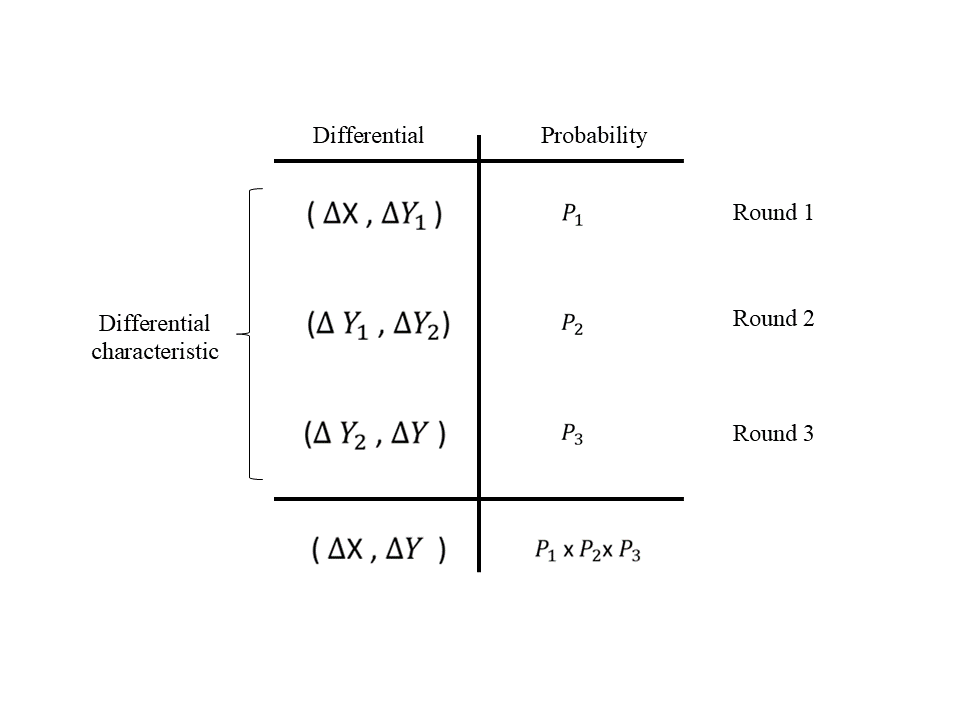
\includegraphics[width=0.9\linewidth]{fig/difchar.png}
    \caption{Concept of constructing differential characteristic}
    \label{fig:difchar}
\end{figure}

\begin{definition}
  DDT is a matrix that tabulates the repetition count of specific output differences $(\Delta Y)$ for all possible input difference $(\Delta X)$ after a single round of a cipher.
\end{definition}
\vspace{1 em}
    \begin{algorithm}[H]
        \DontPrintSemicolon
        Initialize an empty DDT table \\
            \For{$0 \leq dx < 2^{n}-1$}{
                \For {$0 \leq x < 2^{n}-1$}{ 
                    $x1 = dx \oplus x$ \\                    
                    $y = sbox(x)$ \\                  
                    $y1 = sbox(x1)$ \\                    
                    $dy = y \oplus y1 $ \\                    
                    $DDT[dx][dy] += 1$ \\      
                }
            }
        \caption{Pseudocode for DDT }
        \label{alg:ddtkod}
    \end{algorithm}
\vspace{2 em}

With using DDT table we can find differential for each round of the cipher and construct an characteristic for the whole cipher. Stepwise representation for constructing DDT is given in Algorithm \ref{alg:ddtkod} and DDT of cipher PRINCE \cite{borghoff2012prince} is given in table \ref{tbl:ddtprince}

\begin{table}[h!]
\centering
\caption{Differential Distribution Table (DDT) of PRINCE algorithm}
\begin{tabular}{|c|c|c|c|c|c|c|c|c|c|c|c|c|c|c|c|c|}
\hhline{|=|=|=|=|=|=|=|=|=|=|=|=|=|=|=|=|=|}
$\Delta X / \Delta Y $ & 0 & 1 & 2 & 3 & 4 & 5 & 6 & 7 & 8 & 9 & A & B & C & D & E & F \\
\hline
0 & 16 & 0 & 0 & 0 & 0 & 0 & 0 & 0 & 0 & 0 & 0 & 0 & 0 & 0 & 0 & 0 \\
\hline
1 & 0 & 0 & 0 & 0 & 0 & 0 & 0 & 0 & 4 & 4 & 4 & 4 & 0 & 0 & 0 & 0 \\
\hline
2 & 0 & 4 & 0 & 4 & 0 & 4 & 4 & 0 & 0 & 0 & 0 & 0 & 0 & 0 & 0 & 0 \\
\hline
3 & 0 & 0 & 0 & 0 & 0 & 0 & 0 & 0 & 2 & 2 & 2 & 2 & 2 & 2 & 2 & 2 \\
\hline
4 & 0 & 0 & 4 & 0 & 0 & 0 & 2 & 2 & 0 & 0 & 0 & 4 & 2 & 2 & 0 & 0 \\
\hline
5 & 0 & 0 & 4 & 0 & 0 & 0 & 2 & 2 & 0 & 0 & 4 & 0 & 2 & 2 & 0 & 0 \\
\hline
6 & 0 & 2 & 0 & 2 & 2 & 0 & 0 & 2 & 2 & 0 & 2 & 0 & 0 & 2 & 2 & 0 \\
\hline
7 & 0 & 2 & 0 & 2 & 2 & 0 & 0 & 2 & 0 & 2 & 0 & 2 & 2 & 0 & 0 & 2 \\
\hline
8 & 0 & 0 & 0 & 0 & 4 & 4 & 0 & 0 & 0 & 0 & 0 & 0 & 2 & 2 & 2 & 2 \\
\hline
9 & 0 & 0 & 0 & 0 & 4 & 4 & 0 & 0 & 0 & 0 & 0 & 0 & 2 & 2 & 2 & 2 \\
\hline
A & 0 & 0 & 0 & 0 & 0 & 4 & 4 & 0 & 2 & 2 & 2 & 2 & 0 & 0 & 0 & 0 \\
\hline
B & 0 & 4 & 0 & 4 & 0 & 0 & 0 & 0 & 0 & 0 & 0 & 0 & 2 & 2 & 2 & 2 \\
\hline
C & 0 & 0 & 4 & 0 & 0 & 0 & 2 & 2 & 4 & 0 & 0 & 0 & 0 & 0 & 2 & 2 \\
\hline
D & 0 & 0 & 4 & 0 & 0 & 0 & 2 & 2 & 0 & 4 & 0 & 0 & 0 & 0 & 2 & 2 \\
\hline
E & 0 & 2 & 0 & 2 & 2 & 0 & 0 & 2 & 0 & 2 & 0 & 2 & 0 & 2 & 2 & 0 \\
\hline
F & 0 & 2 & 0 & 2 & 2 & 0 & 0 & 2 & 2 & 0 & 2 & 0 & 2 & 0 & 0 & 2 \\
\hline
\end{tabular}

\label{tbl:ddtprince}
\end{table}

The process of differential cryptanalysis can be summarized in 5 steps steps:

\begin{enumerate}
    \item \textbf{Selection of Differentials:}
    \begin{itemize}
        \item Identify differentials $(\Delta X, \Delta Y)$ with non-random propagation probabilities by examining the cipher's S-boxes using the DDT.
        \item Select differentials with highest probabilities.
    \end{itemize}

    \item \textbf{Collection of Pairs:}
    \begin{itemize}
        \item Obtain a large number of plaintext pairs $(P, P')$ such that their XOR difference equals $ \Delta X$.
    \end{itemize}

    \item \textbf{Cipher Execution:}
    \begin{itemize}
        \item Encrypt the selected plaintext pairs through the cipher.
    \end{itemize}

    \item \textbf{Analysis of Output Differences:}
    \begin{itemize}
        \item Analyze the differences in the output ciphertext pairs.
        \item Check if the observed differences match the expected $\Delta Y$.
    \end{itemize}

    \item \textbf{Key Recovery:}
    \begin{itemize}
        \item Use the observed differentials and the associated probabilities to guess parts of the encryption key, focusing particularly on the subkeys used in the last few rounds.
    \end{itemize}
\end{enumerate}


\section{Linear Cryptanalysis}
Originally proposed by Matsui, linear cryptanalysis \cite{matsui1993linear} is a known-plaintext attack applied to the cryptanalysis of block ciphers.The basic methodology of linear cryptanalysis proceeds as follows:

\begin{definition}
A block cipher’s linear approximation can be represented by an equation of the following form:
\begin{equation}
 X[a_1] \oplus X[a_2] \oplus \ldots \oplus X[a_k] \oplus Y[b_1] \oplus Y[b_2] \oplus \ldots \oplus Y[b_l] = 0
\label{eqn:linear}
\end{equation}
\end{definition} 


where $X$ represents the plaintext, $Y$ represents the ciphertext and $a_1, a_2, \ldots, a_k$ and $b_1, b_2, \ldots, b_l$ are bit positions.

Linear cryptanalysis leverages the high probability of certain linear approximations holding over many plaintexts and ciphertexts. In an ideal cipher:
\begin{itemize}
    \item For a given linear approximation, the probability that it holds is $1/2$.
    \item The goal of linear cryptanalysis is to identify linear approximations that occur with probabilities noticeably deviating from $1/2$.
\end{itemize}

Linear cryptanalysis try's to construct equations for each round of the cipher like equation \ref{eqn:linear}. These equations called linear hull.

In order to construct linear approximations for the cipher, we need to find approximations for each round with probabilities significantly different from $1/2$. This involves examining the S-boxes and other nonlinear components of the cipher to determine their linear properties.

\begin{definition}
Within the framework of linear cryptanalysis, the bias of a linear approximation quantifies the deviation of the observed probability of the relation from uniform randomness. It is defined as:
\begin{equation}
bias = \Pr[X_1 \oplus X_2 \oplus \cdots \oplus X_m = Y] - \frac{1}{2}    
\end{equation}
where $X_1, X_2, \ldots, X_m$ are binary variables derived from the plaintext and intermediate values, and $Y$ is the corresponding bit in the ciphertext or an intermediate value. 

\end{definition}
If the probability $\Pr[X_1 \oplus X_2 \oplus \cdots \oplus X_m = Y]$ is $1/2$, then $bias = 0$, indicating that the linear approximation has no bias. A positive or negative bias indicates that the linear approximation occurs more or less frequently than expected under a uniform distribution, respectively. We are trying to construct linear approximation with higher biases. After we found the approxiamtion we need the tool for concatanating them. The Piling-up Lemma is a fundamental result of linear cryptanalysis that describes how the biases of individual linear approximations combine when multiple such approximations are XOR'ed together

\begin{definition}
If  we have $k$ independent linear approximations, then we can calculate their total biases with :
\begin{equation}
total-bias = 2^{k-1} \cdot bias_1 \cdot bias_2 \cdot \cdots \cdot bias_k    
\end{equation}

\end{definition}

This lemma is crucial in evaluating the effectiveness of linear approximations over multiple rounds of a block cipher. It allows to calculate the overall bias of the combined approximations and thereby assess the likelihood of its occurrence, which is vital for constructing an effective linear  attack.

For constructing linear hull, we pass with 1 probability in the linear parts of the cipher. For the non linear parts, we have probabilities. For searching the best linear probabilities we uses LAT tables.

\begin{definition}
The Linear Approximation Table (LAT) is a tool used in linear cryptanalysis to quantify the correlation between linear combinations of input and output bits of an S-box or other cryptographic components. The entry at position $(i, j)$, denoted as $\mathrm{LAT}[i][j]$, represents the bias of the linear approximation for the input mask $i$ and output mask $j$. It is calculated as:

\begin{equation}
\mathrm{LAT}[i][j] = 2 \times \left( \Pr \left[ \bigoplus_{k} i_k \cdot X_k = \bigoplus_{l} j_l \cdot Y_l \right] - \frac{1}{2} \right)     
\end{equation}
   

where $i_k$ and $j_l$ are the bits of the input and output masks, respectively, and $X_k$ and $Y_l$ are the input and output bits of the S-box or function under analysis.
    
\end{definition} 

The LAT provides a comprehensive view of all possible linear approximations for a cryptographic component, allowing cryptanalysts to identify those with the highest biases, which are most useful in a linear cryptanalysis attack. Algorithm \ref{alg:LAT} gives pseudo code for LAT table. Table \ref{tbl:LAT} gives LAT table for SKINNY cipher \cite{beierle2016skinny} . 

\begin{algorithm}[H]
    \DontPrintSemicolon
    \For{$0 \leq \alpha < 2^{n}$}{
        \For {$0 \leq \beta < 2^{n}$}{ 
            \For {$0 \leq x < 2^{n}$}{
                $u = (\alpha \cdot x)$ \\
                $v = (\beta \cdot S(x))$ \\
                \If{$u[0] \oplus ... \oplus u[n] = v[0] \oplus ... \oplus v[n]$}{
                    $LAT[\alpha][\beta]++$
                }
            }
            $LAT[\alpha][\beta] = LAT[\alpha][\beta] - 2^{(n-1)}$
        }
    }
    \caption{Pseudocode for LAT }
    \label{alg:LAT}
\end{algorithm}


\begin{table}[h!]
\centering
\caption{Linear Approximation Table (LAT) of SKINNY cipher.}
\begin{tabular}{|c|c|c|c|c|c|c|c|c|c|c|c|c|c|c|c|c|}
\hhline{|=|=|=|=|=|=|=|=|=|=|=|=|=|=|=|=|=|}
$\alpha \setminus \beta$ & 0 & 1 & 2 & 3 & 4 & 5 & 6 & 7 & 8 & 9 & A & B & C & D & E & F \\
\hline
0 & 8 & 0 & 0 & 6 & 0 & 3 & 6 & -4 & 0 & 6 & 3 & 0 & 6 & 0 & -4 & 8 \\
\hline
1 & 0 & 2 & 2 & 2 & 2 & 1 & 2 & 0 & 2 & 2 & 1 & -2 & 2 & 2 & 0 & 0 \\
\hline
2 & 0 & 2 & 2 & 2 & 2 & 1 & 2 & 0 & 2 & 2 & 1 & -2 & 2 & 2 & 0 & 0 \\
\hline
3 & 6 & 2 & 2 & 6 & 2 & 5 & 6 & -4 & 2 & 4 & 5 & 0 & 6 & 2 & -4 & 6 \\
\hline
4 & 0 & 2 & 2 & 2 & 2 & 1 & 2 & 0 & 2 & 2 & 1 & -2 & 2 & 2 & 0 & 0 \\
\hline
5 & 3 & 1 & 1 & 3 & 1 & 6 & 3 & -1 & 1 & 3 & 6 & 3 & 3 & -1 & -1 & 3 \\
\hline
6 & 6 & 2 & 2 & 6 & 2 & 5 & 6 & -4 & 2 & 4 & 5 & 0 & 6 & 2 & -4 & 6 \\
\hline
7 & -4 & 0 & 0 & -2 & 0 & 1 & -2 & 2 & 0 & -4 & 1 & 0 & -2 & 2 & 2 & -4 \\
\hline
8 & 0 & 2 & 2 & 2 & 2 & 1 & 2 & 0 & 2 & 2 & 1 & -2 & 2 & 2 & 0 & 0 \\
\hline
9 & 6 & 2 & 2 & 6 & 2 & 3 & 6 & -2 & 2 & 4 & 3 & 0 & 6 & 2 & -2 & 6 \\
\hline
A & 3 & 1 & 1 & 3 & 1 & 6 & 3 & -1 & 1 & 3 & 6 & 3 & 3 & -1 & -1 & 3 \\
\hline
B & 0 & -2 & -2 & 0 & -2 & 1 & 0 & 2 & -2 & 2 & 1 & 0 & 0 & -2 & 2 & 0 \\
\hline
C & 6 & 2 & 2 & 6 & 2 & 5 & 6 & -4 & 2 & 4 & 5 & 0 & 6 & 2 & -4 & 6 \\
\hline
D & 0 & 2 & 2 & 0 & 2 & -1 & 0 & 0 & 2 & 2 & -1 & 0 & 0 & 2 & 0 & 0 \\
\hline
E & -4 & 0 & 0 & -2 & 0 & 1 & -2 & 2 & 0 & -4 & 1 & 0 & -2 & 2 & 2 & -4 \\
\hline
F & 8 & 0 & 0 & 6 & 0 & 3 & 6 & -4 & 0 & 6 & 3 & 0 & 6 & 0 & -4 & 8 \\
\hline
\end{tabular}

\label{tbl:LAT}
\end{table}


Using the LAT, we can find linear approximations for each round and construct a linear hull for the whole cipher. The overall process of linear cryptanalysis may be summarized through five key stages.

\begin{enumerate}
\item \textbf{Selection of Linear Approximations:}
\begin{itemize}
\item The first step is to identify potential linear approximations $(\alpha, \beta)$ that describe the relationship between input and output bits of cipher’s S-boxes. These approximations are selected based on their non-random propagation probabilities, which are tabulated in the Linear Approximation Table (LAT).
.
\item After generating the LAT, the linear approximations with the highest biases are selected for further analysis. These approximations are expected to occur with probabilities significantly different from $0.5$, making them useful in distinguishing the cipher from a random permutation and potentially leading to key recovery.
\end{itemize}


\item \textbf{Collection of Pairs:}
\begin{itemize}
    \item In this step, a large number of plaintext-ciphertext pairs $(P, C)$ are collected. The number of pairs required depends on the strength of the bias identified in the LAT. Typically, the more subtle the bias, the more pairs are needed to reliably observe the linear relationship.
    \item The plaintexts can either be chosen or randomly selected, but in either case, the corresponding ciphertexts must be obtained by encrypting these plaintexts using the target cipher. The goal is to have enough data to accurately estimate the probability of the linear approximations.
\end{itemize}

\item \textbf{Cipher Execution:}
\begin{itemize}
    \item Each plaintext in the collected set is encrypted using the cipher, and the resulting ciphertexts are recorded. This step ensures that we have a complete set of plaintext-ciphertext pairs, which is essential for the statistical analysis in the following steps.
    \item The linear approximations that were selected in the first step are then applied to these pairs. Specifically, for each pair, the input and output linear combinations specified by $(\alpha, \beta)$ are calculated and compared.
\end{itemize}

\item \textbf{Analysis of Linear Approximations:}
\begin{itemize}
    \item This step involves analyzing how often the selected linear approximations hold true across the collected pairs. For each pair, we check if the linear approximation $(\alpha \cdot P) \oplus (\beta \cdot C) = 0$ holds, where $\alpha \cdot P$ represents the dot product of $\alpha$ with the plaintext bits, and $\beta \cdot C$ represents the dot product of $\beta$ with the ciphertext bits.
   
\end{itemize}

\item \textbf{Key Recovery:}
\begin{itemize}
    \item Last step is to use observed linear approximations with their associated biases to make educated guesses about the key bits, particularly those taking place in the final rounds of the cipher. Since the linear approximations are most likely to hold true for the correct key, the attacker can systematically test different key hypotheses and compare how well they align with the observed data.
    \item By focusing on the subkeys from the last rounds, the attacker can incrementally limit the number of possible keys, leading to the recovery of the entire encryption key with reduced computational effort compared to brute-force.
\end{itemize}

\end{enumerate}

\section{Related-Key Differential Cryptanalysis}

Related-key differential cryptanalysis \cite{biham1994new} is an advanced form of differential cryptanalysis that exploits the relationships between the keys used in a cipher. Introduced by Biham , this attack is based on the premise that in some cryptographic systems, different keys may produce outputs with predictable differences when the same plaintext is encrypted under these keys.

\subsection{Principle of Related-Key Differential Cryptanalysis}

The core concept of related-key differential cryptanalysis is to study the differential behavior of a block cipher when  related keys are used. Instead of relying only on plaintext differences as in standard differential cryptanalysis, this technique considers the differences between keys, which are applied to the same plaintext or ciphertext.

Let $K$ and $K^*$ be two related keys, where $K^*$ is derived from $K$ by applying a known difference $\Delta_K$. The goal is to find a differential characteristic that holds with a high probability when the same plaintext $P$ is encrypted under both $K$ and $K^*$. The resulting ciphertexts $C$ and $C^*$ should then have a predictable difference $\Delta C$.

Formally, a related-key differential characteristic can be expressed as:

$$
\Delta_K \rightarrow \Delta_P \rightarrow \Delta_C
$$

Where:
\begin{itemize}
    \item $\Delta_K = K \oplus K^*$ is the key difference.
    \item $\Delta_P = P \oplus P^*$ is the plaintext difference.
    \item $\Delta_C = C \oplus C^*$ is the ciphertext difference.
\end{itemize}

The attack involves finding such a differential characteristic that holds with a high probability over multiple rounds of the cipher, enabling the cryptanalyst to exploit this relationship for key recovery.

\subsection{Steps in Related-Key Differential Cryptanalysis}

The process of performing related-key differential cryptanalysis is generally carried out in the following steps:

\begin{enumerate}
    \item \textbf{Key Difference Selection}:
    \begin{itemize}
        \item The first step is to select an appropriate key difference $\Delta_K$. This step often involves analyzing the key schedule to understand how key differences propagate.
    \end{itemize}
    
    \item \textbf{Differential Characteristic Identification}:
    \begin{itemize}
        \item Next, the attacker identifies a differential characteristic that describes how the plaintext difference $\Delta_P$ and the key difference $\Delta_K$ propagate through the cipher to produce a predictable ciphertext difference $\Delta_C$. The characteristic is chosen such that the probability of the differential characteristic holding over the rounds of the cipher is high.
    \end{itemize}
    
    \item \textbf{Plaintext-Ciphertext Pair Collection}:
    \begin{itemize}
        \item The attacker collects pairs of plaintexts and their corresponding ciphertexts under both keys $K$ and $K^*$. These pairs are then analyzed to determine if the expected differential characteristic is observed. How many pairs are needed depends on the characteristic’s probability as well as the computational complexity of the attack.
    \end{itemize}
    
    \item \textbf{Key Recovery}:
    \begin{itemize}
        \item By analyzing the observed differences and comparing them with the expected differential characteristic, the attacker can make educated guesses about the key bits, especially those involved in the last few rounds of the cipher. By testing various hypotheses, the attacker narrows down the possible values of the key, ultimately recovering the encryption key.
    \end{itemize}
\end{enumerate}






